
\setcounter{chapter}{5-1}

\chapter{Feature Representation}

    \subsection*{What's still missing?}
    
        Last chapter, we used our linear regression model to do classification: we created a "hyperplane" to \textbf{separate} the the data that we placed in each class. 
    
        We also mentioned that regularization can increase \textbf{structural error}, by limiting what possible $\theta$ models we're allowed to use. 
            \note{Our goal was to decrease estimation error, but that's beside the point right now.}
    
        But, what if our linear model is already \textbf{too limited}? What if we need a more complicated model? This is true in a lot of real-world problems, like vibration:
    
        \begin{figure}[H]
            \centering
            
            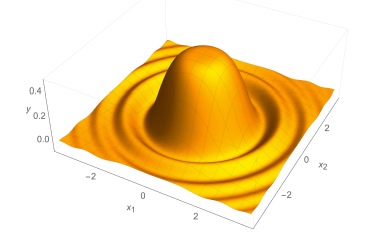
\includegraphics[width=70mm,scale=0.5]{images/feature_images/nonlinear_example.png}
            \caption*{This wave doesn't seem particular friendly to a planar approximation.}
        \end{figure}
    
        These kinds of situations are called, appropriately, \textbf{non-linear}.\\
    
        \begin{concept}
            \vocab{Non-linear} behavior cannot be accurately represented by any \gren{linear} model. 
    
            In order to create an accurate model, we have to use some \purp{nonlinear} operation.
        \end{concept}
    
        If we could create effective, non-linear models, we might even be able to deal with data that was previously "\textbf{linearly inseparable}".

    \subsecdiv

    \subsection*{Possible Solutions: Polynomials}

        Let's try to think of ways to approach this problem. We'll start with a 1-D input, for simplicity.

        Upon hearing "non-linear", we might remember the function we introduced last chapter: the \textbf{sigmoid}.
    
        \begin{figure}[H]
            \centering
            
            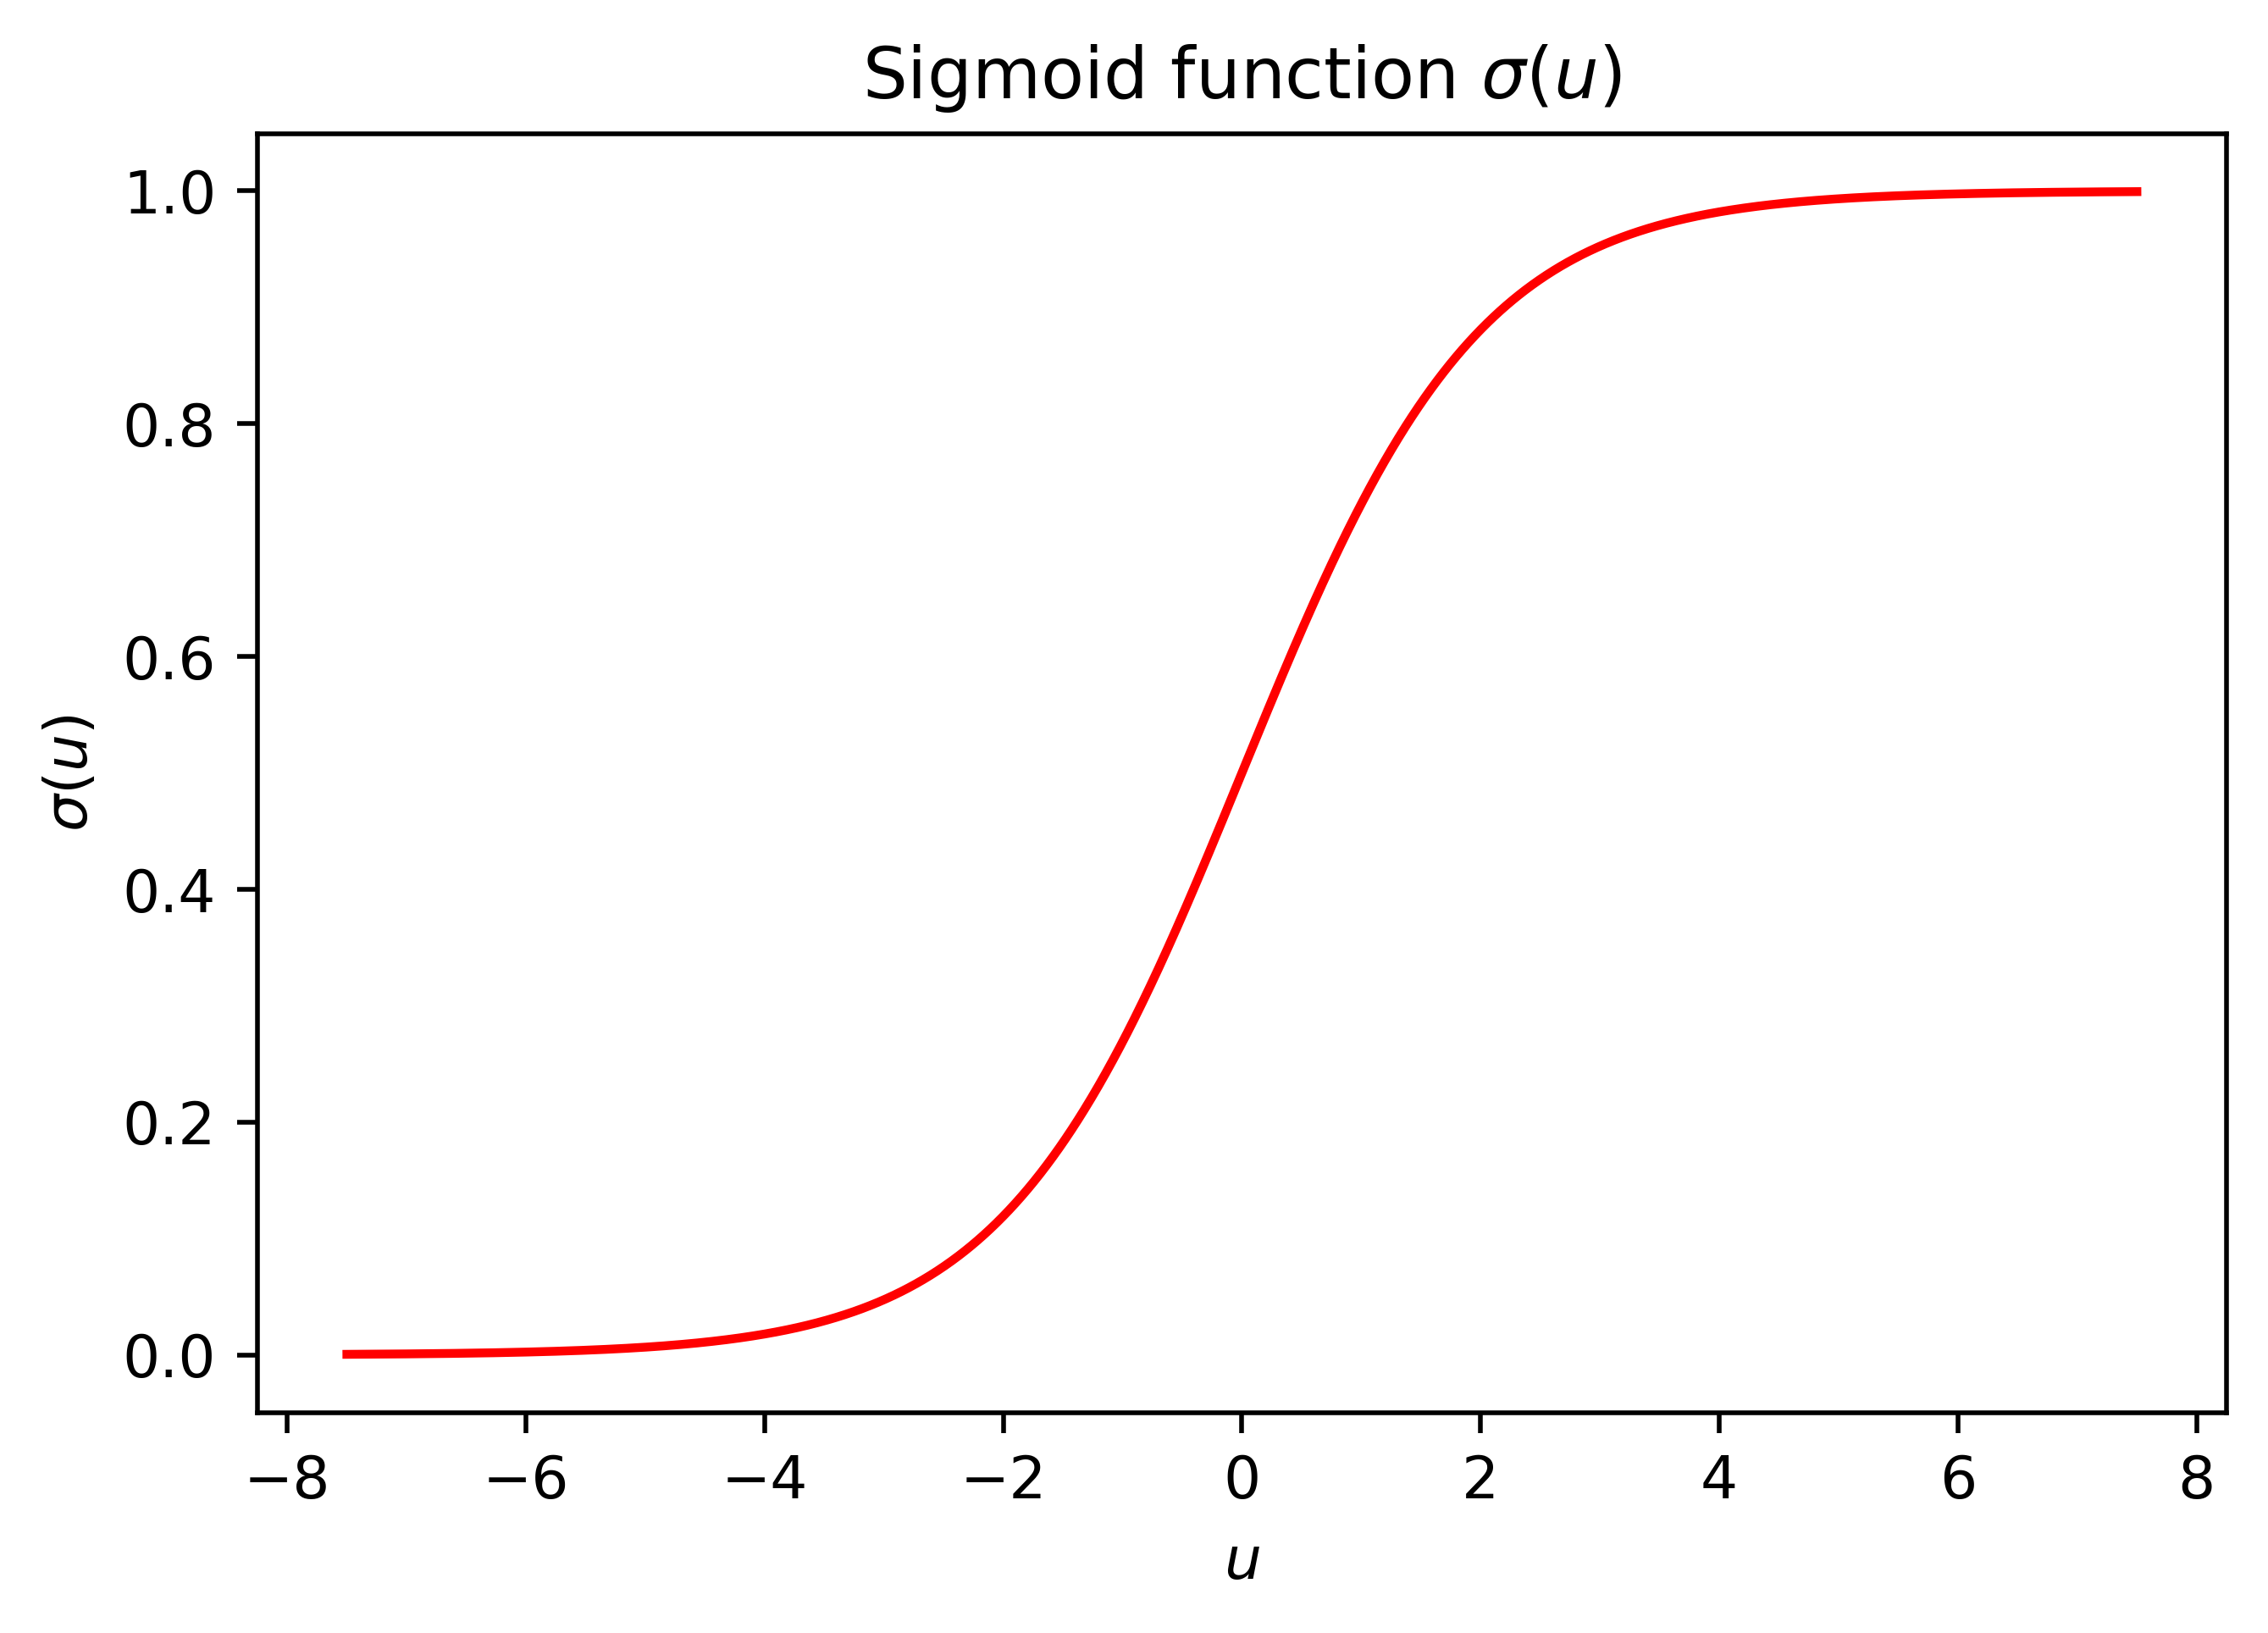
\includegraphics[width=70mm,scale=0.5]{images/feature_images/sigmoid_u.png}
            \caption*{Your friendly neighborhood sigmoid.}
        \end{figure}
    
        Can we use this to create a new model class? For now, unfortunately not: remember that we used this in the last chapter, and we still got a \textbf{linear} separator. The reasons were discussed there.
            \note{We'll show ways we can use this kind of approach, when we discuss Neural Networks.}
    
        Instead, we can get inspiration from our example of "structural error". For now, let's focus on \orgg{regression} (though classification isn't too different):
    
        \begin{figure}[H]
            
            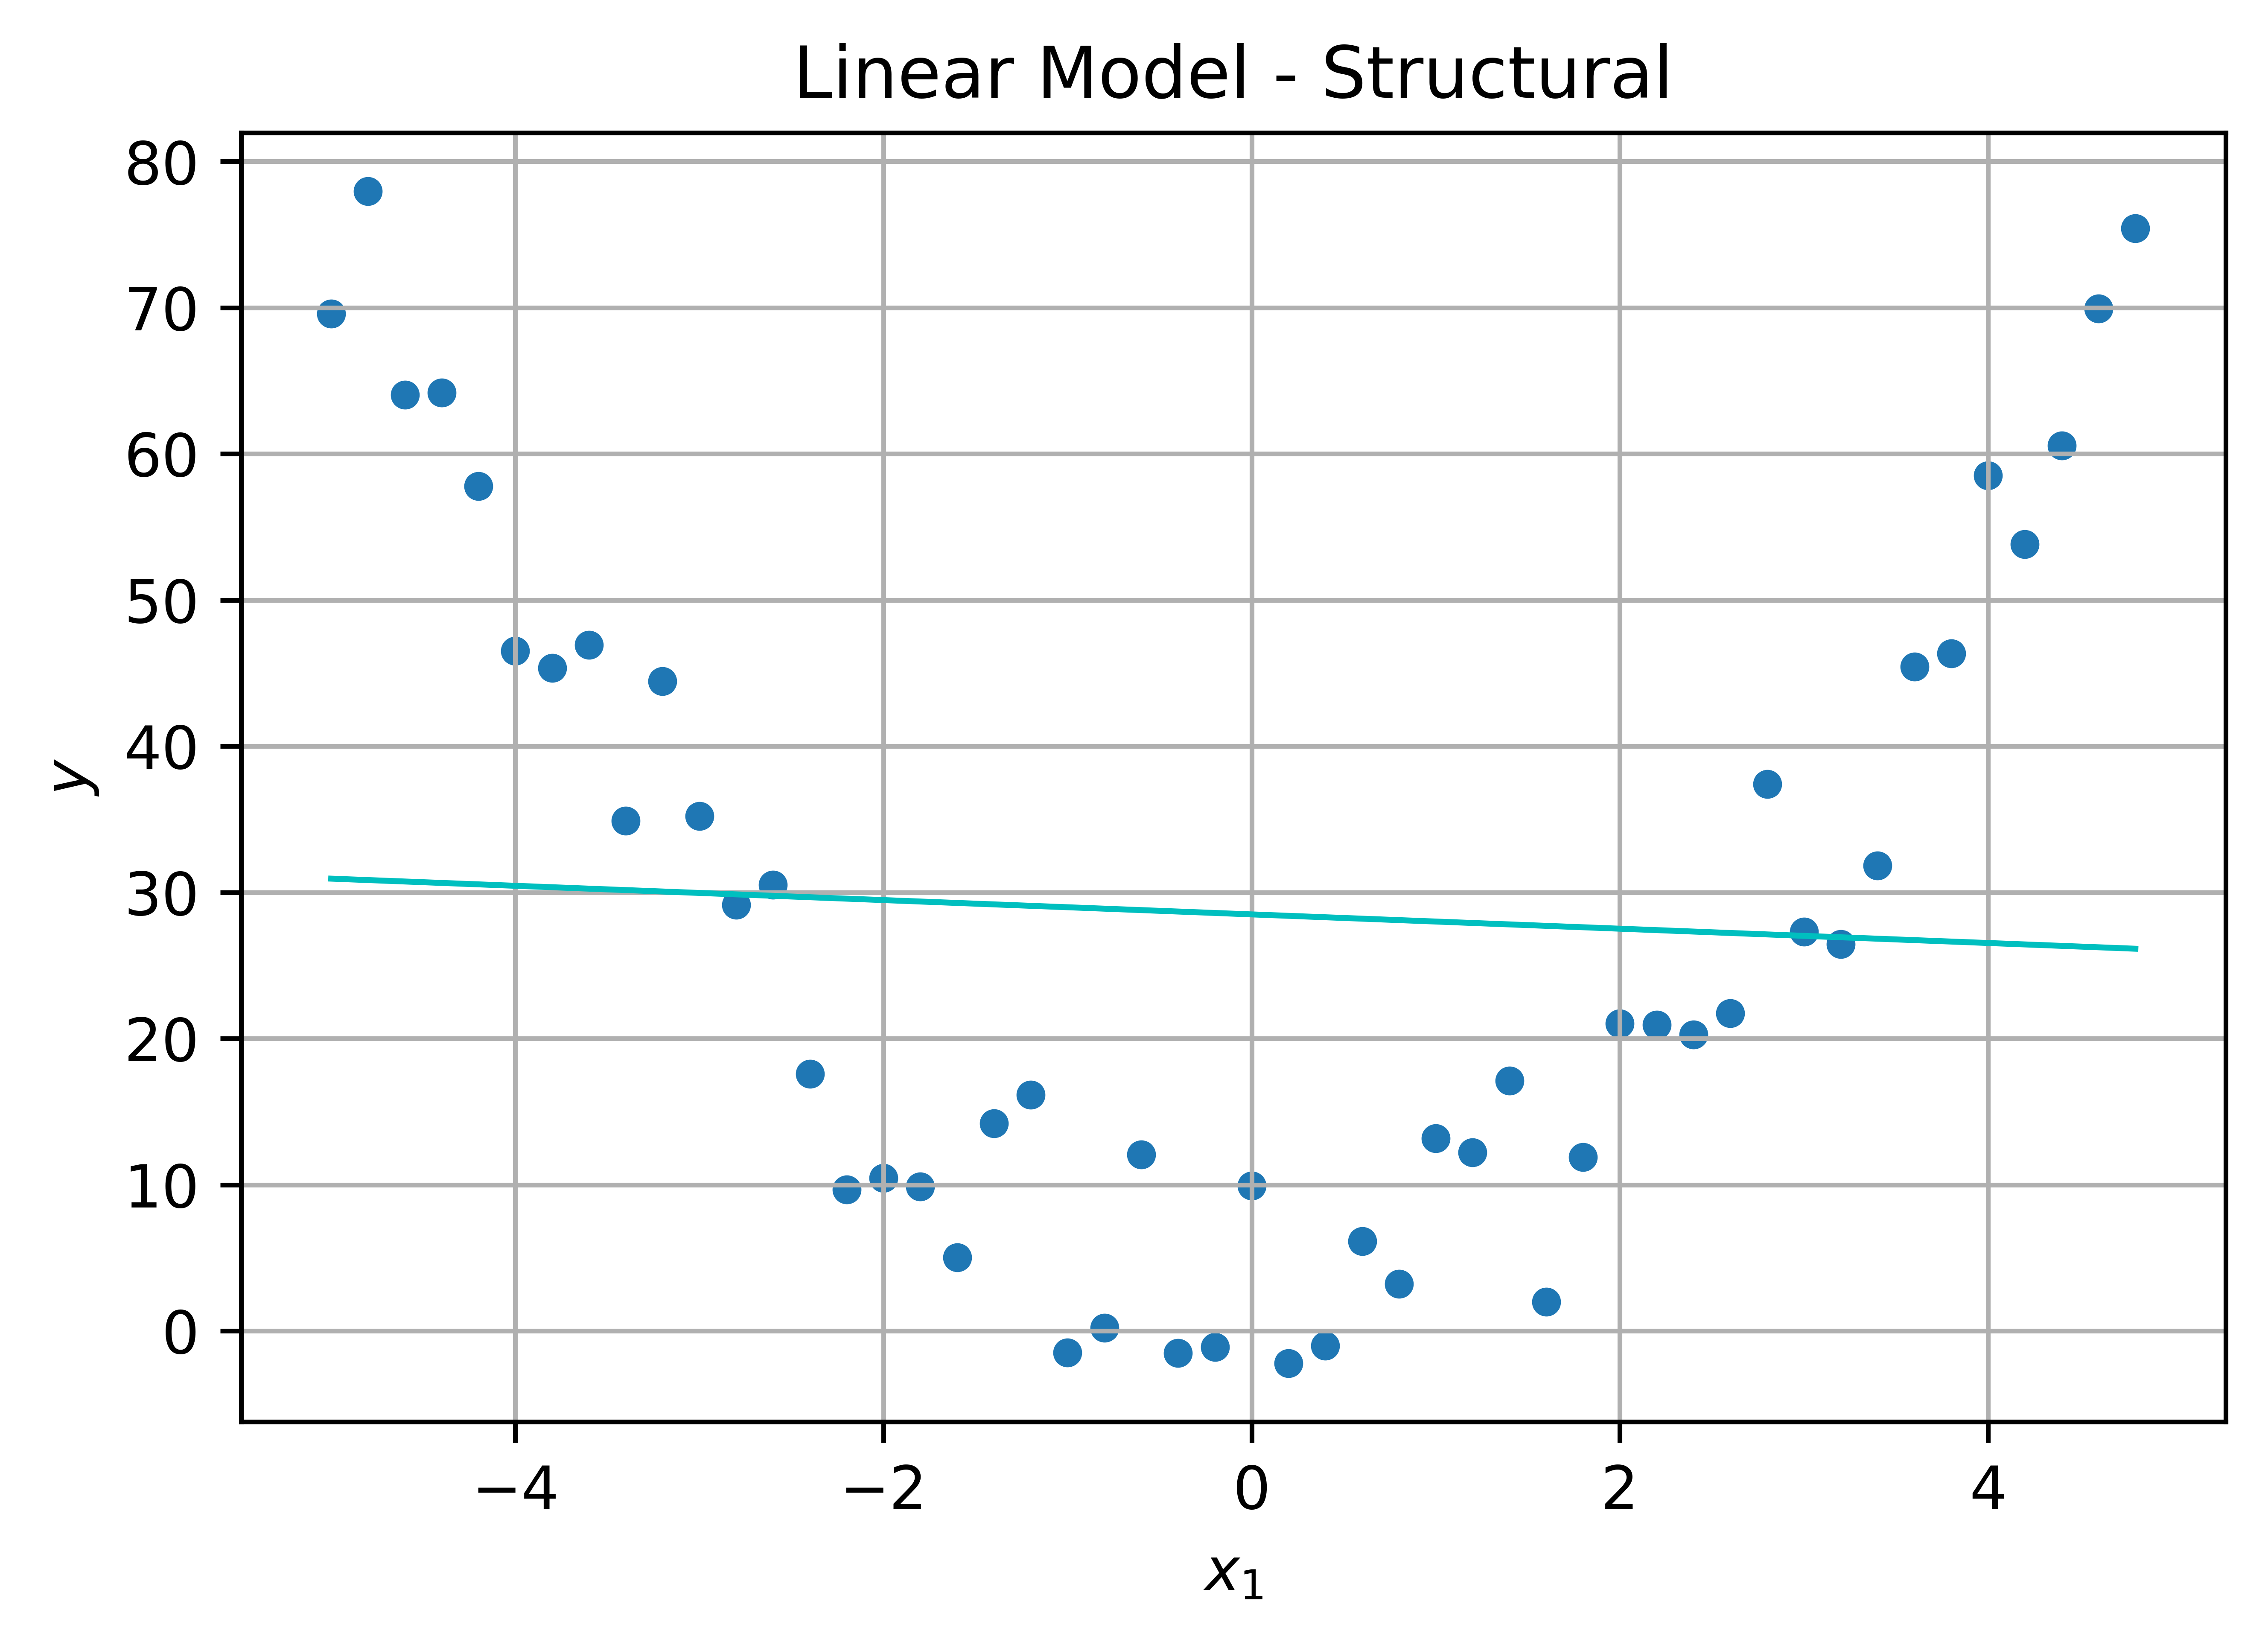
\includegraphics[width=70mm,scale=0.5]{images/feature_images/Structural_Linear_Model.png}
            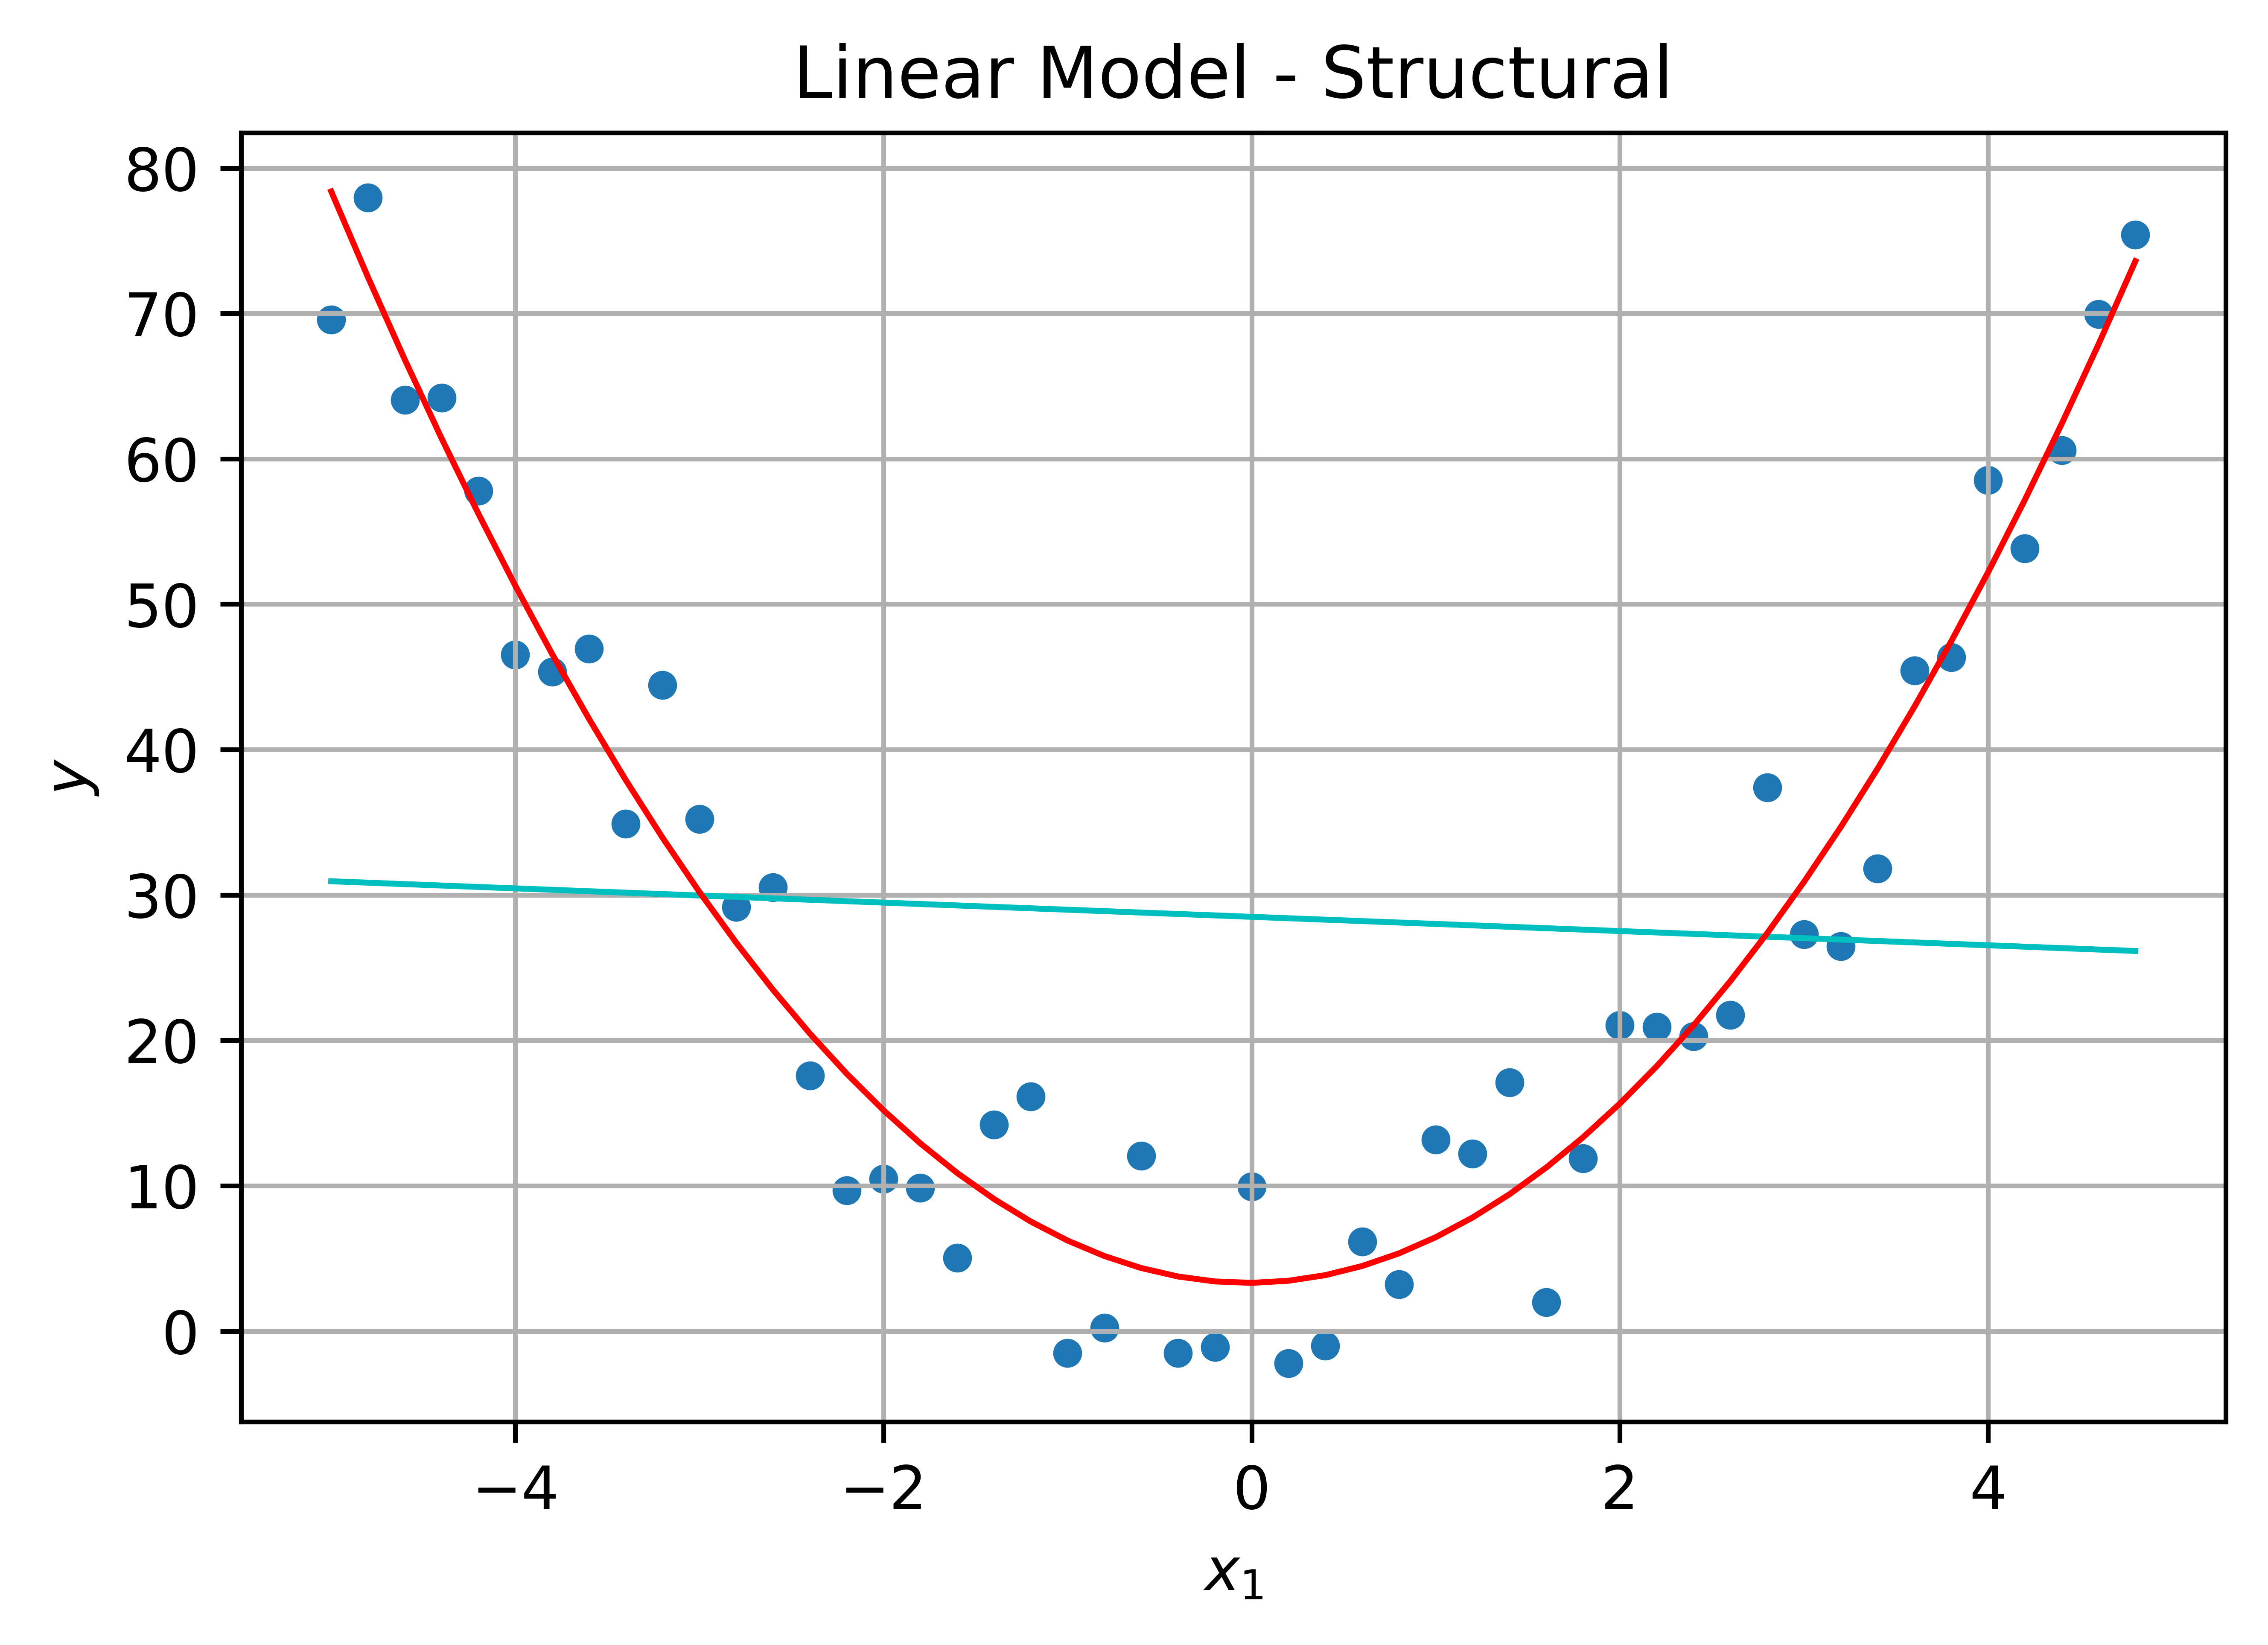
\includegraphics[width=70mm,scale=0.5]{images/feature_images/Structural_Quad_Model.png}
    
            \caption{A linear regression can't represent this dataset. However, a parabola can!}
        \end{figure}
    
        We're still using our input variable $x$, but this time, we've "\textbf{transformed}" it: we have squared $x$, giving us a model of the form
            \note{Remember that $x$ is 1-D right now!}
    
        \begin{equation}
            h(x) = \red{A}x^2+\red{B}x+\red{C}
        \end{equation}
    
        It should be clear that his model is more \textbf{expressive} than the one before: it can create every model that our linear approach could (just by setting $A=0$), and it can create new models in a parabola shape.
            \note{Reminder: "expressiveness" or "richness" of a hypothesis class is how many models it can represent: a more expressive model can handle more different situations.}\\
    
        \begin{concept}
            We can make our \purp{linear} model more \gren{expressive} by add a squared term, and turning it into a \purp{parabolic} function.
    
            This concept can be extended even further, to any \orgg{polynomial}.

            This is called a \vocab{polynomial transformation} of our input data.
        \end{concept}

    \subsecdiv
    
    \subsection*{Transformation}
    
        How do we \textit{generalize} this concept? Well, we have a set of constant parameters $A, B, C$. These are similar to our constants $\theta_i$. Let's change our notation:
    
        \begin{equation}
            h(x) = \red{\theta_2} x^2 + \red{\theta_1} x + \red{\theta_0}
        \end{equation}
    
        Now, we've got something more familiar. We could imagine extending this to any number of terms $\theta_i x^i$: if we needed a cubic function, for example, we could include $\theta_3 x^3$.

        This is starting to look pretty similar to our previous model: in fact, we could even separate out $\theta$ as a parameter:
            \note{Notice that $\theta_0$ corresponds to $x^0=1$.}

        \begin{equation}
            h(x) = 
            \overbrace{
                \sum_{i=1}^{k}
                \theta_i x^i
            }^{\text{Polynomial sum}}
            =
            \overbrace{
            \begin{bmatrix}
             \theta_0 \\ \theta_1 \\ \theta_2 \\ \vdots \\ \theta_k
            \end{bmatrix}
            \cdot 
            \begin{bmatrix}
                1 \\ x \\ x^2 \\ \vdots \\ x^k
            \end{bmatrix}
            }^{\text{Store as vectors}}
            = 
            \overbrace{
            \theta^T
            }^{\text{Simplify}}
            \begin{bmatrix}
                1 \\ x \\ x^2 \\ \vdots \\ x^k
            \end{bmatrix}
        \end{equation}

        This really \textit{is} starting to look like our linear transformation $\theta^T x$. That's helpful: we might be able to use the techniques we developed before.

        In fact, we can argue that they're \textbf{equivalent}: we've just changed what our input vector is. Consider our new input $\phi(x)$:
            \note{Compare the structure of $\theta^T x$ versus $\theta^T \phi(x)$: you've replaced $x$ with $\phi(x)$.}

        \begin{equation}
            \blu{\phi(x)}
            = 
            \begin{bmatrix}
                1 \\ x \\ x^2 \\ \vdots \\ x^k
            \end{bmatrix}
            \qquad \qquad
            h(x) = 
            \red{\theta^T} 
            \overbrace{
            \blu{\phi(x)}
            }^{\text{New input}}
        \end{equation}
        
        This is called \textbf{transforming} our input. However, polynomial is only one of our transformations!\\

        \begin{definition}
            A \vocab{transformation} $\phi(x)$ takes our input vector $x$ and converts it into a \gren{new} vector.

            This transformation can be used to:

            \begin{itemize}
                \item Allow our model to handle new, more \gren{complex} situations 
                
                    \begin{itemize}
                        \item \miniex Polynomial transformations
                    \end{itemize}

                \item \gren{Pre-process} our data to make certain \gren{patterns} more obvious, and easy for our model to detect.

                    \begin{itemize}
                        \item \miniex Radial transformations (to be discussed later!)
                    \end{itemize}
                
                \item Convert our data into a \gren{usable} format (if the original format doesn't fit into our equations)

                    \begin{itemize}
                        \item \miniex One-hot encoding
                    \end{itemize}
                
            \end{itemize}
        \end{definition}

        \miniex Taking our input $x$ and converting it into a polynomial is a \textbf{transformation} of our input.

        This chapter will focus on these kinds of transformations. 

    \subsecdiv

    \subsection*{Features}
        
        One benefit of only changing the input is that everything else we know about the model is still true: we can continue to use our linear representation.
            \begin{itemize}
                \item We will be able to optimize a "linear" model $\theta$, over data that has been made \textbf{nonlinear}.
            \end{itemize}

        These transformations can be complex, especially for \orgg{multi-dimensional} inputs. In this first case, we only combined one input ($x=x_1$) with \textbf{itself}. But, often, we can combine multiple $x_i$ together!
            \note{We'll cover this multi-dimensional polynomial transformation later in the chapter.}

        So, we need to be careful of our input variables $x_i$. 
        
        \begin{itemize}
            \item We sometimes call a single input variable, a single "\textbf{feature}". However, we need to be careful: this word can have multiple meanings.\\
        \end{itemize}

        \begin{clarification}
            We often use the word \vocab{feature} in related (but not identical) contexts:

            \begin{itemize}
                \item A \vocab{feature} can be one unprocessed \gren{aspect} of the \purp{data}: 
                    \begin{itemize}
                        \item \miniex Whether or not something is a cat or a dog, or the height of a patient.
                    \end{itemize}

                \item A \vocab{feature} can also be one mathematical \gren{variable} in our \purp{transformed input}. 
                    \begin{itemize}
                        \item $x_i$ is a \gren{feature} of the \orgg{data}.
                        \item $\phi(x)_j$ (one variable in $\phi(x)$) is a \gren{feature} of the \orgg{transformed data}.
                    \end{itemize}
            \end{itemize}

            Just like how we have an \redd{input space} and a \redd{hypothesis space}, we call the collection of possible values for our features the \redd{feature space}.
        \end{clarification}
    
        Combined, this is why we called this technique the \textbf{feature transformation}: 
            \begin{itemize}
                \item We apply a transform to the \textbf{features} $x$ of our data, and create a new list of \textbf{features} $\phi(x)$.
            \end{itemize}

        Since these transforms only apply to our features, they don't affect the rest of our model. So, we can still use \textbf{linear} tools:\\

        \begin{definition}
            \vocab{Feature transformation} allows us to do \gren{linear} regression or classification on a list of \purp{features} we have \gren{non-linearly} \purp{transformed}:

            \begin{equation*}
                h(x) = 
            \red{\theta^T} 
            \blu{\phi(x)}
            \end{equation*}

            \begin{itemize}
                \item The $\theta^T u$ operation is still linear $(u=\phi(x))$.
                \item All non-linearity is stored in $\phi(x)$.
            \end{itemize}
        \end{definition}

    \secdiv

    \pagebreak

    \section{Gaining intuition about feature transformations}

        Now that we understand the general idea of feature transformations, we can begin work with them, particularly for \orgg{classification}.

        Our goal is often to take data that linear models couldn't handle, and make them \textbf{more accurate}.

        So, we'll consider maybe the simplest (solvable) case of a nonlinear data set in 1-D:
            \note{The y-axis doesn't exist, it just has vertical height to make it easier to view on a page.}

        \begin{figure}[H]
            \centering
            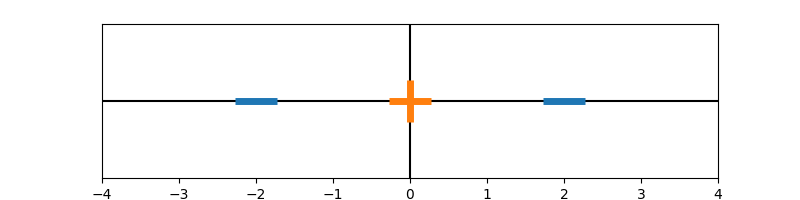
\includegraphics[width=120mm,scale=0.5]{images/feature_images/inseparable.png}
            \caption{In this state, there's no 0-d plane (point) that would \textbf{separate} these data points.}
        \end{figure}

        This is where our transform comes in: we can't separate using just $x$. So, we'll introduce a second variable: $x^2$.
            \note{We're replacing 

                \phantom{}
                
                $\theta x + \theta_0 >0$ with 

                \phantom{}
                
                $\theta_2x^2 + \theta_1 x + \theta_0>0$.}

        \begin{itemize}
            \item We want a function that lets us classify some data points as positive, and some as negative.
            \item For the dataset in this image, $-x^2+2>0$ gives us 100\% accuracy. Let's see it in action:
                

            \begin{center}
                    \begin{tabular}{c || c || c}
                    $x=2$ & y= $-(2)^2+2 = -2$ & $y<0 \implies Negative$ \\
                    $x=0$ & $y = -(0)^2+2 = 2$ & $y>0 \implies Positive$ \\
                    $x=-2$ & $y= -(-2)^2+2 = -2$ & $y<0 \implies Negative$ \\
                    \end{tabular}
                \end{center}
                
        \end{itemize}

        How do we visualize this? It turns out, there are different perspectives:\\

        \begin{clarification}
            There are \gren{two} different ways we can \vocab{graph} a transformation:

            We transform the \purp{hyperplane}:
            
            \begin{itemize}
                \item \miniex If our model is \orgg{$f(x)=-x^2+2$}, we just graph $y=f(x)$ as our separator in 2D space.
                    
                    \begin{itemize}
                        \item This is the approach we used to start the chapter: we wanted a line that \gren{fit} to our data.
                        \item In practice, this bends our \gren{hyperplane} into a curve: at the start of the chapter, we transformed a line into a parabola.
                    \end{itemize}
            \end{itemize}
            
            Or, we transform the \purp{data}:
            
            \begin{itemize}
                \item \miniex We plot each data point in 2D as \orgg{$[x, -x^2+2]$}.
                    \begin{itemize}
                        \item This model allows us to keep a "\gren{linear} separator": we "shift" the data nonlinearly, \textbf{then} linearly separate it.
                    \end{itemize}
            \end{itemize}

            These models are mathematically \gren{equivalent}, and we'll switch the approach we're using based on which is easier/more useful to graph.
        \end{clarification}

            \note{See our plot examples for each below.}

        Note that our nonlinear transformation "adds" dimensions: we had a 1D problem, and we used a second dimension to separate it.

        It may seem concerning to transform the \textbf{data}, rather than the \textbf{model}. The data is what we're using to make decisions, after all. 
        
        However, keep in mind that:

        \begin{itemize}
            \item Our model already was a sort of \orgg{transformation}: even the linear model $\theta$ "transforms" each data point $x$ into $y=\theta^T x$.
            
            \item Usually, we try to preserve the \gren{original structure} of the data, so we don't lose information: we just add more.
                \begin{itemize}
                    \item For example, $[1,x,x^2]$ still contains the information $x$: we just append 1 and $x^2$.
                \end{itemize}
        \end{itemize}

        \miniex Let's show both of these in action, using the 1-D dataset we showed above.

        \subsecdiv

        \subsection{Transforming our separator}
    
            First, we transform our linear separator as desired: graphing $-x^2+2=f(x)$.

            \begin{itemize}
                \item Our separator points are still on the x-axis: they "separate" our data wherever $f(x)=0$.
            \end{itemize}
    
            \begin{figure}[H]
                \centering
                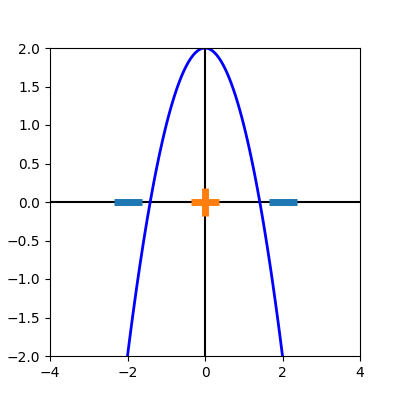
\includegraphics[width=60mm,scale=0.5]{images/feature_images/nonlinear_separator.png}
                \caption*{In this version, we've taken our hyperplane separator and transformed it nonlinearly.}
            \end{figure}
    
            To correctly classify, we assign $-x^2+2>0$ as positive.
    
            In this version, we preserve the structure of the data, making it easier to see the original shape. 

            However, it's not as easy to think about the direction and orientation of the "plane" now that it's been deformed into a parabola. 
            
            \begin{itemize}
                \item For example, we don't really have a good "normal" vector, even if we know which side is positive.
            \end{itemize}
            
            This is why, to keep our model "linear", we can transform the \textbf{data}, instead of the separator. We'll do that next.
    
            \subsecdiv

        \subsection{Transforming our data}
    
            In this case, every data point gets plotted on $[x,x^2]$. Our hyperplane is given by 
    
            \begin{equation}
                -x^2+2 =\;
                \overbrace{
                \red{\begin{bmatrix}
                    0 \\ -1
                \end{bmatrix}^T}
                }^{\theta^T}
                \blu{\begin{bmatrix}
                    x \\ x^2
                \end{bmatrix}}
                + 2
                =
                \red{\theta^T}\blu{\phi(x)} + \theta_0
            \end{equation}
    
            Thus, we get a $\theta$ plane pointing downward, with an offset of 2.
    
            \begin{figure}[H]
                \centering
                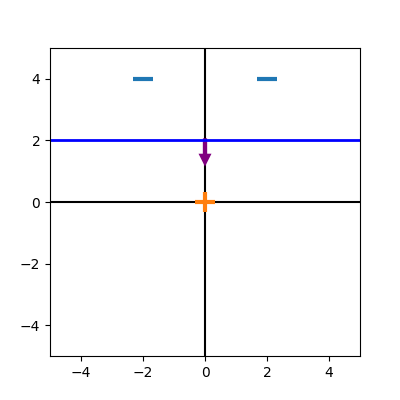
\includegraphics[width=60mm,scale=0.5]{images/feature_images/nonlinear_data.png}
                \caption*{This time, we've transformed our data: the math is totally the same, but now we can identify our separator more easily.}
            \end{figure}
    
            Note that our transformation makes the data linearly separable!\\
    
            \begin{concept}
                Features transformations allow us to \purp{non-linearly} transform our data, in order to make that data \gren{linearly separable}, or at least, more \gren{accurate} with a linear separator.
    
                Often, we do this by transforming into a \purp{higher dimensional} space.
            \end{concept}
    
            \subsecdiv

        \subsection{Positive vs. Negative}

            While these perspectives are helpful, they can become too complicated with more dimensions/higher-dimensional transformations.

            In an effort to simplify, we might ask ourselves, "what do we really want to know"? In the end, all we typically care about is classification: which data points are positive or negative?

            So, we'll create a third representation to correspond to that.\\

            \begin{concept}
                A third, \gren{simplified} representation of our transformation doesn't show how it affects our data points or classifier. Instead, we just show the \purp{result}: which regions are classified as positive, and which are classified as negative?

                This allows us to see which points get \gren{classified} in which way, without considering the high-dimensional details of the model itself.
            \end{concept}

            \miniex We can graph this for our sample data:

            \begin{figure}[H]
                \centering
                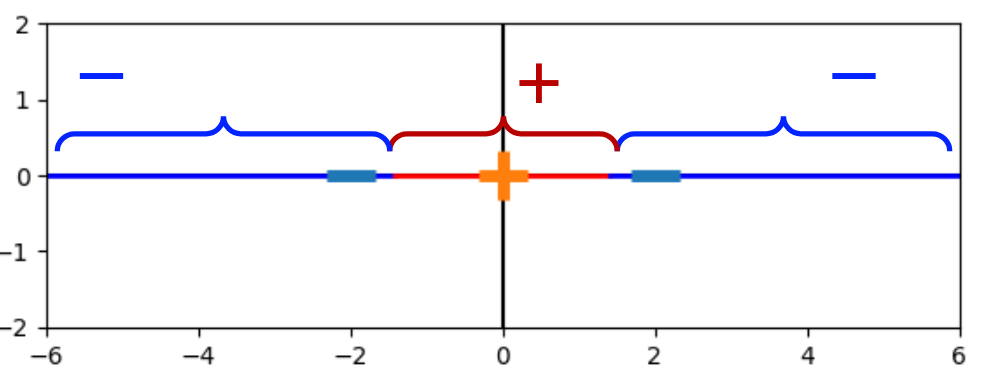
\includegraphics[width=100mm,scale=0.5]{images/feature_images/positive_negative_disp.png}
                \caption*{This way, we can stay in a 1-D space, while showing the information we need!}
            \end{figure}

            Note that the points where we switch between positive and negative, $\pm \sqrt{2}$, are the points corresponding to $-x^2+2=0$: they're the only part of the separator surface visible in our 1D plot.
                \note{They match our nonlinear hyperplane separator from section 5.1.1}


        \secdiv

    \pagebreak

    \section{Systematic feature construction}

        Now that we've established feature transformations, let's consider a couple options for how we'd want to do it, and how we can generalize to higher dimensions. 

        Here, we'll present two common ways to construct features, in a way that's consistent across problems, or "systematic".
            \note{We could also call this "problem independent": it works regardless of what kind of problem you have. Though, that doesn't mean problem type won't affect performance.}

        \subsection{Polynomial Basis}

            At the start of this chapter, we introduced the idea of polynomial transformations.
            
            If a linear function isn't "expressive" enough to solve a problem, then we can create a more complex model, based on how many $x^i$ we include. This can be written as:

            \begin{equation}
                h(x) =
                \sum_{i=1}^{k}
                \red{\theta_i} \blu{x^i}
                =
                \red{
                \begin{bmatrix}
                 \theta_0 \\ \theta_1 \\ \theta_2 \\ \vdots \\ \theta_k
                \end{bmatrix}
                }
                \cdot
                \blu{
                \begin{bmatrix}
                    1 \\ x \\ x^2 \\ \vdots \\ x^k
                \end{bmatrix}
                }
                =
                \red{\theta_0} + \red{\theta_1}\blu{x^2} + \red{\theta_2}\blu{x^2} + \cdots + \red{\theta_k}\blu{x^k}
            \end{equation}

            Another word for these $x_i$ terms might be a "polynomial \textbf{basis}".

            \begin{itemize}
                \item Why call it a basis? Well, we can use our $x_i$ terms to create a polynomial, using
            \end{itemize}

            \begin{equation}
                \sum_i \theta_i x^i
            \end{equation}

            \begin{itemize}
                \item Using this procedure, we can combine \gren{basic} elements $x_i$ to create any \gren{polynomial}.
            \end{itemize}

            \begin{equation}
                \setty{1, x_1, x_2, \cdots x_k}
            \end{equation}

            \begin{itemize}
                \item This is what defines it as a \purp{basis}: the ability to combine these terms, make any polynomial we want.
            \end{itemize}
            

    
            
            \subsubsection{Order}
            
                An important question to ask is, "how many terms do we include"?

                We categorize our polynomials based on the highest exponent included: this is called the \textbf{order}.\\

                \begin{definition}
                    \vocab{Order} $k$, also known as \vocab{degree}, is the \purp{largest} exponent allowed in our \gren{polynomial}. 

                    Every higher exponential $x^{j}$ can be thought of as having a coefficient $\theta_k=0$: as far as we're concerned, it \gren{doesn't exist}.
                \end{definition}

                \miniex We can compare different orders, by looking at the feature vector they create.
                    \note{Note that, while we chose every coefficient to be nonzero here, they don't have to be! $-x^2+2$ from before is a valid second-order polynomial.}

                Here's a table of the first few:\\

                \begin{center}
                    \begin{tabular}{c c c}
                    Order & $d=1$ & Example \\
                    \hline
                    0 & $[1]$ & $\red{3.5}$  \\
                    1 & $[1,x]^T$ & $\red{2.5x}-1$ \\
                    2 & $[1,x,x^2]^T$ & $\red{4.1x^2}-10x+1$ \\
                    3 & $[1,x,x^2,x^3]^T$ & $\red{x^3}+8x^2+x-\sqrt{2}$ \\
                    $\vdots$ & $\vdots$ & $\vdots$ \\
                    k & $[1, x, x^2, \cdots, x^k]$ & $\sum_{j=1}^k \theta_jx^j$ \\
                    $\vdots$ & $\vdots$ & $\vdots$
                    \end{tabular}
                \end{center}

                \phantom{}

                The order we choose is an important design choice.
                
            \subsecdiv

            \subsubsection{Overfitting with order}
                It's difficult to know how many terms to include in our polynomial, but we run into two problems if our order is \textbf{too high}:

                \begin{itemize}
                    \item It becomes time-consuming to calculate, with little benefit
                    \item We start overfitting more and more.
                \end{itemize}

                The first part makes sense: with more terms, we have to do more multiplications, more additions, etc.\\
                
                \begin{concept}
                    More \vocab{complex models} tend to be more \purp{expensive} to train, and slower to use. This is a trade-off for more \gren{accuracy}. 
                    
                    Usually, there's a point where cost \gren{outweights} benefits. A problem is rarely perfectly solved, even by an excellent model, so you can't just continue until it's "perfect".
                \end{concept}

                But what about the second part? Why do we increase overfitting? 

                With a higher order, our polynomial becomes more complex: it can take on more shapes, which are increasingly complex and perfectly fit to the data.

                This can cause our data to overlook obvious patterns, and instead create a very precise shape that is paying attention to the noise in our model.\\

                \begin{concept}
                    \vocab{High-order polynomials} are very vulnerable to \purp{overfitting}.

                    Because they can take on so many different, \gren{complex} functions, they can very very closely \purp{match} the original data set. 
                    
                    This can cause the model to "learn" noise, and \gren{miss} broader and simpler patterns that actually exist. In may fail to learn something broad and useful, while \purp{memorizing} the dataset with its expressiveness.
                \end{concept}

                Let's see this in action: we'll generate some data based on $2x+1$, while applying some random noise to it. We'll see the optimized linear regression model for each.
                    \note{For ease, we'll exclude regularization: it does help mitigate this problem, but it doesn't totally solve it.}

                Rather than transform the data, we'll transform the separator: this really highlights the overfitting effect.

                \begin{figure}[H]
                    \centering
                    
                    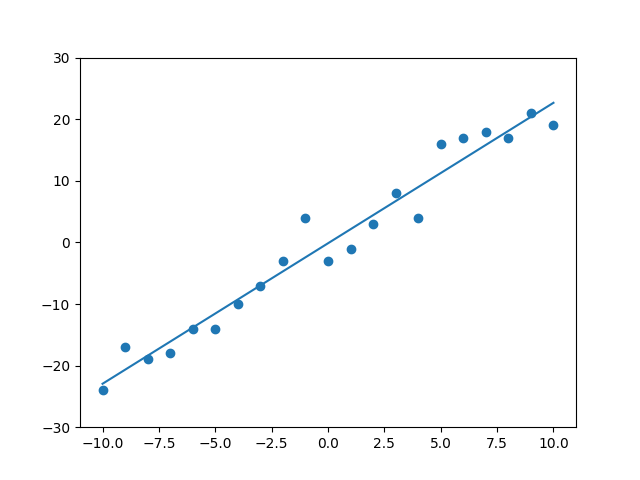
\includegraphics[width=70mm,scale=0.5]{images/feature_images/order_1_soln.png}
                    \caption*{Here's the 1st order solution: in this case, correct for the underlying distribution. It fits our data fine.}
                \end{figure}

                \begin{figure}[H]
                    \centering
                    
                    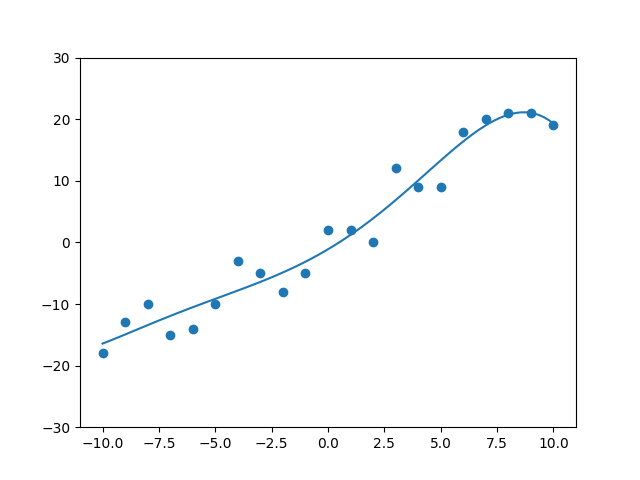
\includegraphics[width=60mm,scale=0.5]{images/feature_images/order_5_soln.png}
                    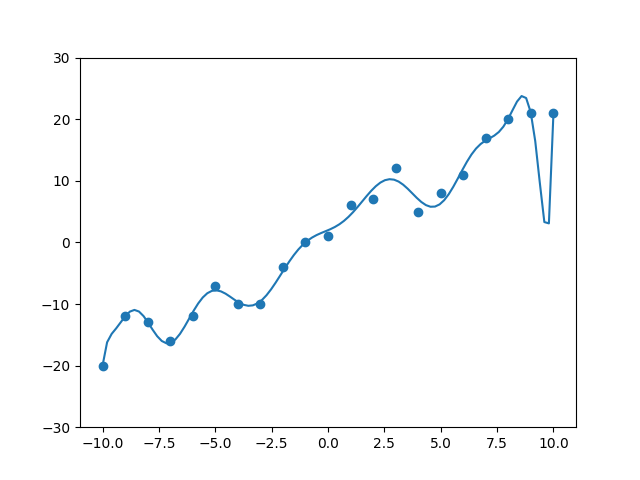
\includegraphics[width=60mm,scale=0.5]{images/feature_images/order_15_soln.png}
                    \caption*{5th and 15th order. The left model looks suspicious, and the right is way overfit. It's very unlikely that we know such an intricate pattern, from so little data.}
                \end{figure}

                 \begin{figure}[H]
                    \centering
                    
                    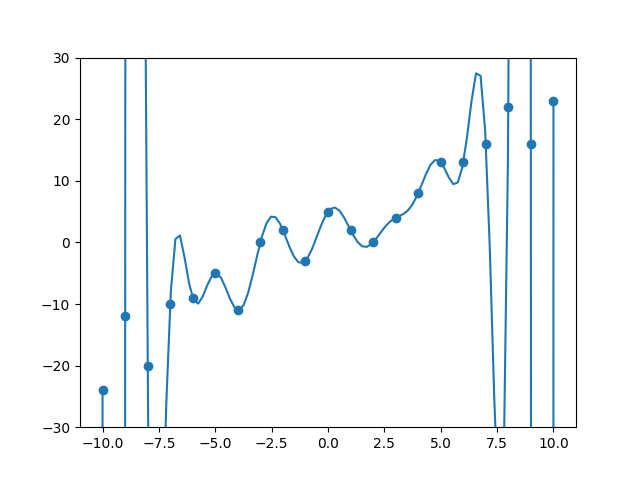
\includegraphics[width=70mm,scale=0.5]{images/feature_images/order_20_soln.png}
                    \caption*{20th order. We have one order for each data point: now, our model is capable of doing regression going through every single data point: as overfit as physically possible, perfectly matching the data.}
                \end{figure}

            \subsecdiv
            \subsubsection{Higher dimensions}

                Until now, we've only been focusing on the 1-D case of data. Let's change that. Let's consider a 2D dataset $[x_1,x_2]^T$.

                We start with our typical 2D model:

                \begin{equation}
                    \theta^Tx + \theta_0 = \theta_1x_1 + \theta_2x_2 + \theta_0
                \end{equation}

                Is polynomial basis, with "order 1": the largest exponent is 1. This is still a "linear" model.

                \subsecdiv

                If we want to move up to order 2, we increase the \gren{largest exponent}, adding $x_1^2$ and $x_2^2$ to the basis.

                However, this doesn't take full advantage of the expressiveness of our model: this only creates parabolas aligned with the $x_1$ and $x_2$ axes. How do we create other options?

                Well, we created these options by multiplying $x_1$ with another $x_1$. It seems like we could logically expand to multiplying $x_1$ by $x_2$.\\

                \begin{definition}
                    For \vocab{higher dimension} $d>1$ \vocab{polynomials}, we allow for multiplication \purp{between variables} $x_i$ and $x_j$.

                    The \vocab{order} of the polynomial is the maximum number of times you can \purp{multiply variables} together. 
                    
                    For order $k$, the \gren{sum of exponents} must be \purp{less than or equal to} the order.
                \end{definition}

                So, for $d=2$, order=$2$, we get the basis:

                \begin{equation}
                    \begin{bmatrix}
                        1 & \red{x_1} & \red{x_1^2} & \blu{x_2} & \blu{x_2}\red{x_1} & \blu{x_2^2}
                    \end{bmatrix}^T
                \end{equation}

                For $d=2$, order=$3$, it starts getting a bit messy: we have 10 different basis terms.
                    \note{You don't need to memorize these.}

                \begin{equation}
                    \begin{bmatrix}
                        1 & x_1 & x_1^2 & x_1^3 &
                        x_2 & x_2x_1 & x_2x_1^2 & x_2^2 &
                        x^2x_1 & x^3
                    \end{bmatrix}^T
                \end{equation}

            \subsecdiv
            \subsubsection{Total number of features}
        
                How many do we have in general? Well, every term results from multiplying variables \textbf{at most} $k$ times. Or, the exponents \textbf{add up} to at most $k$.
                
                If we count 1 as a factor, we can say that the exponents always add up to $k$ (since $1^j$ has no effect). So, we have $d+1$ different numbers, which add up to exactly $k$.
                    \note{We have $d$ variables, so $d+1$ if we include 1 as a variable.}

                For example, here's how this would look for $d=2$, $k=2$ (5.10 above). All you need to notice is that the exponents add to 2.

                \begin{equation}
                    \begin{bmatrix}
                        1^{\pur{2}}x_2^{\blu{0}}x_1^{\red{0}} & 1^{\pur{1}}x_2^{\blu{0}}x_1^{\red{1}} & 
                        1^{\pur{0}}x_2^{\blu{0}}x_1^{\red{2}} & 1^{\pur{1}}x_2^{\blu{1}}x_1^{\red{0}} & 1^{\pur{0}}x_2^{\blu{1}}x_1^{\red{1}} & 
                        1^{\pur{0}}x_2^{\blu{2}}x_1^{\red{0}}
                    \end{bmatrix}^T
                \end{equation}


                This is a well-known problem in combinatorics: how many ways are there to add up $d+1$ numbers to total $k$? The solution to this problem gives us:
                    \note{Explaining the math here is beside the point of this course. If you're curious, search up "stars and bars math", or visit \href{https://en.wikipedia.org/wiki/Stars_and_bars_(combinatorics)}{here}.}

                \begin{equation}
                    \binom{(d+1)+k-1}{k} = \binom{d+k}{k} = \frac{(d+k)!}{d!k!}
                \end{equation}

            \subsecdiv
            \subsubsection{Summary of Polynomial Basis}

                \phantom{}

                \begin{definition}
                    The \vocab{polynomial basis} of order $k$ and dimension $d$ includes \purp{every feature}

                    \begin{equation*}
                        \prod_{i=1}^d x_i^{c_i}
                    \end{equation*}

                    Where all of the integer exponents $c_i\geq 0$ add up to \gren{at most} $k$.

                    Creating features such as:

                    \begin{equation*}
                        x_1^k, \;\; x_1x_2, \;\; x_2x_3^3x_6, \;\; 1, \;\; \dots
                    \end{equation*}
                \end{definition}

                We can represent this in a table:
                    \note{This table is different from the one we saw earlier!}

                \begin{center}
                    \begin{tabular}{c c c}
                    Order & $d=1$ & in general ($d>1$) \\
                    \hline
                    0 & $[1]$ & \blu{$[1]$}\\
                    1 & $[1,x]^T$ & \blu{$[1,x_1, \ldots, x_d]^T$}\\
                    2 & $[1,x,x^2]^T$ & \blu{$[1,x_1, \ldots, x_d,
                                        x_1^2, x_1x_2, \ldots]^T$}\\
                    3 & $[1,x,x^2,x^3]^T$ & \blu{$[1,x_1, \ldots,
                                        x_1^3, x_1x_2, \ldots,
                                        x_1x_2x_3, \ldots]^T$} \\
                    $\vdots$ & $\vdots$ & $\vdots$ \\
                    \end{tabular}
                \end{center}

            \subsecdiv


        \subsubsection{Polynomial Basis in Action}

            Below, we'll show examples of how polynomial basis being used, to demonstrate just how useful it is.

            But how do we use feature transformations? The best part: remember that we can view it as a linear separator? We can train it just the same way!\\

            \begin{concept}
                \vocab{Feature transformations} \purp{don't change} how we train our model. We can still treat our model as a \gren{linear} vector $\theta$, even if our data has been \gren{non-linearly} transformed. 

                So, after we transform our data, we can use normal techniques (OLS, gradient descent, SGD) to fit our model.
            \end{concept}

            In this situation, the benefits of regularization become more clear: by preventing $\theta$ from becoming too large, we discourage a surface that is too "extreme", with larger changes across its surface.

            We'll train our model for various situations, to see what it can do. Different problems require different orders $k$, still.
            
            \begin{figure}[H]
                \centering
                
                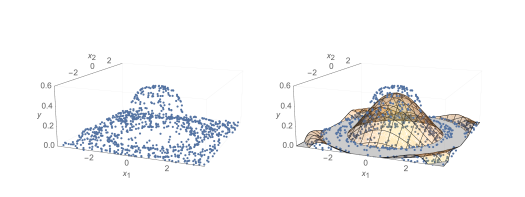
\includegraphics[width=80mm,scale=0.5]{images/feature_images/vibrations.png}
                \caption*{We start with the waveform we showed at the start of the chapter: on the left, we see a bunch of datapoints we want to take a regression over. With $k=8$, we get a pretty good result.}
            \end{figure}

            For 2D separators, it's easier to show only the +/- classification, rather than the transformed data/boundary. That means, these below graphs are hiding the numeric outputs.
            
            Light indicates "positive" for the model, dark indicates "negative" for the model.

            \begin{figure}[H]
                \centering
                
                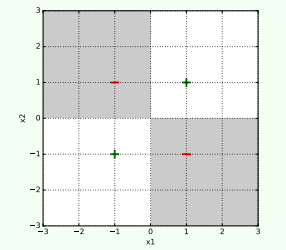
\includegraphics[width=70mm,scale=0.5]{images/feature_images/xor.png}
                \caption*{This is the classic "xor" problem: a typical case of "linearly unseparable". With $k=2$, we can classify it well with the chosen model $4x_1x_2=0$.}
            \end{figure}

            \begin{figure}[H]
                \centering
                
                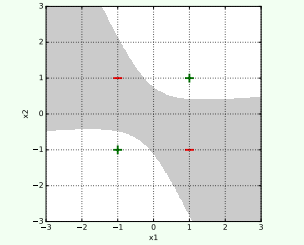
\includegraphics[width=70mm,scale=0.5]{images/feature_images/better_xor.png}
                \caption*{This time we use gradient descent and a random initialization to get a less rigid, but still effective classification. }
            \end{figure}

             \begin{figure}[H]
                \centering
                
                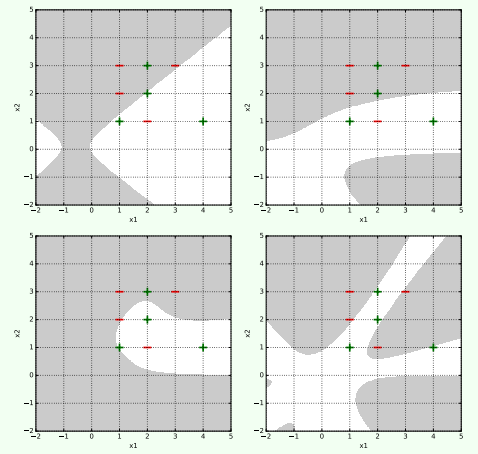
\includegraphics[width=70mm,scale=0.5]{images/feature_images/harder_dataset.png}
                \caption*{This dataset is pretty brutal: we try with $k=2,3,4,$ and finally $5$. The shapes we get are... complex, to say the least. But, we successfully solve it with $k=5$.}
            \end{figure}

        \subsecdiv
        \subsection{Radial Basis}

            Finally, we consider an alternative way to create a feature space.

            \begin{itemize}
                \item With the "polynomial basis" approach, we \textbf{combined features} to create more complex surfaces to \textbf{fit} the structure of the data.
                
                \item This "radial basis" approach, on the other hand, \textbf{combines data points} to \textbf{learn} more about the structure of the data.
            \end{itemize}

            What do we mean by that? Well, let's consider what we mean by "structure": when we're judging data, what sorts of patterns are we looking for?

            Often, we're looking to see, "what data is near/similar to other data?" Similar data is more likely to behave similarly, after all.
                \note{We'll come back to these ideas when we talk about clustering!}

            So, it might be useful to include distance between data points as a feature: how do we implement this? Well, let's do this one-by-one: we'll create a feature for the distance to a single data point $p$.
            
            We start with squared distance, for smoothness reasons.

            \begin{equation}
                ||p-x||^2
            \end{equation}

            This feature would \textit{grow} as data points get further apart, though. We want to see what data is \textit{close}: the opposite.

            We could use a function like $\frac{1}{u}$. However, this would explode to infinity as distances shrink: not good.

            $e^{-u}$ is a better fit: it approaches 1 when $u=0$, and, relatedly, it tends to drop off more smoothly and gradually than $1/u$. 

            Finally, we add a coefficient $\beta$ to the exponent to give us more control: it will tell us how quickly our function decays with distance.
                \note{The word "decay" is used commonly for exponential decrease.}\\

            \begin{definition}
                We define the \vocab{radial basis function}

                \begin{equation*}
                    f_{ \red{p} }(x) = e^{-\beta ||\red{p}-x||^2 }
                \end{equation*}

                As a \purp{feature} in the RBF feature transformation.

                This transformation takes a data point $p$ and provides a feature $f_p(x)$ that represents "\gren{closeness}" of $x$ to $p$.
            \end{definition}

            Note some useful properties of this transform:
            \begin{itemize}
                \item For small distances, this feature creates a \textbf{connection} between $p$ and our data point: representing some local "structure" of \textbf{closeness}.
                \item If points are far away, this effect gradually \textbf{vanishes}: points which are \textbf{far} away have very little to do with each other.
                \item $\beta$ controls what is considered "close" and "far": 
                    \begin{itemize}
                        \item if $\beta$ is large, points have to be very close for an effect.
                        \item if $\beta$ is small, we have a larger "neighborhood" of points with a relevant $f_p(x)$.\\
                    \end{itemize}
            \end{itemize}

            \begin{definition}
                The \vocab{radial basis functions (RBF)} transform takes each of the data points in the input, and uses it to create a set of \purp{radial basis function} features. 

                Collectively, they make the \gren{feature space}:

                \begin{equation*}
                    \phi(x) = 
                    \Big[
                    f_{\red{\ex{x}{1}}}(x), \;\; 
                    f_{\red{\ex{x}{2}}}(x), \;\; 
                    \cdots, \;\; 
                    f_{\red{\ex{x}{n}}}(x)
                    \Big]^T
                \end{equation*}

                Where:

                \begin{equation*}
                    f_{\red{p}}(x) = e^{-\beta ||\red{p}-x||^2 }
                \end{equation*}

                This transform allows us to represent "closeness" within our dataset. With it, we can compare new data points to some "reference" points $\ex{x}{i}$.
                
                It's often used to allow us to represent our dataset in a way that is approximate, but still useful.
            \end{definition}

            This general idea is useful for problems like:
            \begin{itemize}
                \item Function approximation,
                \item Optimization,
                \item Reducing noise in signals
                    \note{Reminder that "noise" just refers to anything undesired in the signal. Usually added by randomness or the environment.}
            \end{itemize}

            This approach is not limited to the "squared distance" idea of closeness, either: if you can come up with another way to define distance, you can use the same approach.
                \note{These ways to define distance are called "distance metrics".}

            
    \secdiv
    


            
    \pagebreak
    \section{Hand-constructing features for real domains }

        So far, we've focused on transformations that handle two of our main problems (which have a lot of overlap):
            \note{Borrowed from the transformation definition above.}

        \begin{itemize}
                \item Allow our model to handle new, more \textbf{complex} situations (more \textbf{expressiveness})

                \item \textbf{Pre-process} our data to make it \textbf{easier} for our model to find \textbf{patterns}.
                
            \end{itemize}

        Now, we'd like to turn our attention to the last of the three:

        \begin{itemize}
            \item Convert our data into a \textbf{usable} format (if, say, the original format doesn't fit into our equations)
        \end{itemize}

        One challenge with our models are they rely on computation and calculation. This usually require our input to be something like a \textbf{number}.

        But we don't always receive data in this way: words, brands, colors, and odd others data types, are often presented instead. Frequently, we even need to \textbf{adjust} our numerical inputs.

        The \textbf{transformations} in this section address these kinds of problems. We take data that is informative, but not currently usable, and converting them to something we can \textbf{compute} with.\\

        \begin{concept}
            Often, we have to \vocab{convert} between data types, in order to do the machine learning work we want to do.

            This requires using the appropriate \purp{transforms} to get data we can work with, without \gren{losing} important \gren{information}.
        \end{concept}

        As mentioned above, we have to be \textbf{careful}: if we use the wrong data type, we can \textbf{lose} crucial information that our model could have made use of.

        \subsecdiv

        \subsection{Discrete Features}

            One of the most common issues with data types is figuring out what to do with \textbf{discrete} features: ones that are broken up into categories.

            These categories may or may not have an order, or some other important information. We need to use the right data type to keep as much information as possible. This will allow our model to more easily discover patterns.

            We'll make the following assumption:\\

            \begin{clarification}
                In this textbook/course, we assume that all \purp{input vectors} $x$ should be \gren{real-valued vectors} (or: $x \in \R^d$)
            \end{clarification}


            And now, we go through some common examples of feature transformations:

            \subsubsection{Numeric}

                First, we consider the case where our pre-processing \textbf{feature} is "\textit{almost}" in a number format: each class could reasonably correspond to a \textbf{number}.\\
    
                \begin{definition}
                    In the \vocab{numeric} transformation, we convert each of our $k$ classes into a \purp{number}. 
    
                    \begin{itemize}
                        \item This approach is only appropriate if each class is roughly "numeric": it fits appropriately into the \gren{real numbers}.
                            \begin{itemize}
                                \item We have a clear \purp{ordering}, and
                                \item The numbers have the \purp{structure} of real numbers: \gren{distance} between points, or the idea of \gren{adding/multiplying}, makes sense.
                            \end{itemize}
                    \end{itemize}
                \end{definition}

                \miniex There are many ways to do this. Here, we evenly distribute values evenly between 0 and 1:
                    \note{Remember: which way you transform should reflect the nature of your data!}
    
                    \begin{equation}
                        \begin{bmatrix}
                            \frac{1}{k} & \frac{2}{k} & \cdots & \frac{k-1}{k} & 1
                        \end{bmatrix},
                        \qquad 
                        \text{Class } i \longrightarrow \frac{i}{k}
                    \end{equation}

            \subsecdiv
            \subsubsection{Thermometer Code}

                Next, we'll relax how number-like our feature is. This time, we don't need our data to behave like a number, but it does have an \textbf{ordering}.
                    \note{By "relax", we mean we'll remove some requirements for our feature, like being able to add them together.}

                Some examples:

                \begin{itemize}
                    \item Results of an opinion poll:
                        \begin{itemize}
                            \item "Strongly Agree", "Agree", "Neutral", "Disagree", "Strongly Disagree"
                        \end{itemize}
                    
                    \item Education level: 
                        \begin{itemize}
                            \item "Below High School", "High School Degree", "Associates Degree", "Bachelors" "Advanced Degree"
                        \end{itemize}
                    
                    \item Ranking of athletes
                \end{itemize}

                In this case, we can't just use numbers $\{1,2,3,...\}$. Why not?

                Because that implies that there's a specific "scaling" between points: Is the \#1 athlete twice as good as the \#2 athlete? Maybe, but that's not what the ranking tells us!\\

                \begin{concept}
                    Data that is \vocab{ordered} but not \purp{numerical} cannot be represented with \gren{a single real number}.

                    Otherwise, we might consider one element to be a certain amount "larger" or "smaller" than another, when that's not what \gren{ordering} means.
                \end{concept}

                \miniex Suppose we assign $\{1,2,3\}$ for $\{Disagree, Neutral, Agree\}$. The person who writes 'agree' is doesn't "agree three times as much" as the person who writes 'disagree'!

                But, we still want to keep that ordering: counting up from one element to the next. How do create an order without creating an exact, numeric difference?

                Just now, we tried to count by increasing a single variable. But, there's another way to count: counting up using multiple different variables!
                    \note{This approach is more similar to counting on your fingers.}

                \begin{equation*}
                    \text{Class 1} \longrightarrow
                    \begin{bmatrix}
                        \blu{0} \\ \blu{0} \\ \blu{0} \\ \red{1}
                    \end{bmatrix}
                    \qquad \;\;
                    \text{Class 2} \longrightarrow
                    \begin{bmatrix}
                        \blu{0} \\ \blu{0} \\ \red{1} \\ \red{1}
                    \end{bmatrix}
                    \qquad \;\;
                    \text{Class 3} \longrightarrow
                    \begin{bmatrix}
                        \blu{0} \\ \red{1} \\ \red{1} \\ \red{1}
                    \end{bmatrix}
                    \qquad \;\;
                    \text{Class 4} \longrightarrow
                    \begin{bmatrix}
                        \red{1} \\ \red{1} \\ \red{1} \\ \red{1}
                    \end{bmatrix}
                \end{equation*}
                
                This version allows us to avoid the problems we had before: this doesn't behave the same way as a \textbf{numerical} value.

                To better understand what's going on, here's another way to frame it:
                    \note{Class$(x)$ is just shorthand for, "which class is $x$ in?"}

                \begin{equation}
                    \phi(x) =
                    \begin{bmatrix}
                        \text{Class}(x)\geq 4 \\
                        \text{Class}(x)\geq 3\\
                        \text{Class}(x)\geq 2\\
                        \text{Class}(x)\geq 1
                    \end{bmatrix}
                \end{equation}

                \miniex Suppose $x$ is in class 3. The bottom three statements are all true, the top one is false: so we get $[0, 1, 1, 1]^T$. 

                This helps us understand why this encoding is so useful:
                
                \begin{itemize}
                    \item We aren't directly "adding" variables to each other: they stay separated by \textbf{index}.
                    
                    \item When using a linear model $\theta^T\phi(x)$, each class  matches a different $\theta_i$.
                        \note{$\theta_i$ scales the $\nth{i}$ variable. So, each class can be scaled differently!}
                        
                    \item Despite not behaving like numbers, "higher" classes in the order still keep track of all of the classes "below" them.
                        \begin{itemize}
                            \item \miniex Class 2-4 all share the feature $\text{Class}(x)\geq 2$ (equivalent to $\text{Class}(x)>1$).
                        \end{itemize}
                \end{itemize}

                This technique is called \textbf{thermometer encoding}.\\

                \begin{definition}
                    \vocab{Thermometer encoding} is a \purp{feature transform} where we take each class and turn it into a feature vector $\phi(x)$ where

                    \begin{equation*}
                    \text{Class 1} \longrightarrow
                    \begin{bmatrix}
                        \blu{0} \\ \vdots \\ \blu{0} \\ \blu{0} \\ \red{1}
                    \end{bmatrix},
                    \qquad 
                    \text{Class 2} \longrightarrow
                    \begin{bmatrix}
                        \blu{0} \\ \vdots \\ \blu{0} \\ \red{1} \\ \red{1}
                    \end{bmatrix}
                    \qquad
                    \text{Class 3} \longrightarrow
                    \begin{bmatrix}
                        \blu{0} \\ \vdots \\ \red{1} \\ \red{1} \\ \red{1}
                    \end{bmatrix}
                    \qquad
                    \text{Class } k \longrightarrow
                    \begin{bmatrix}
                        \red{1} \\ \vdots \\ \red{1} \\ \red{1} \\ \red{1}
                    \end{bmatrix}
                \end{equation*}

                    \begin{itemize}
                        \item The \purp{length of the vector} is the \gren{number of classes} $k$ we have.
                        \item The $\nth{i}$ class has $i$ \purp{ones}.
                    \end{itemize}

                    \subsecdiv

                    \begin{itemize}
                        \item This transformation is only appropriate if the data 
                            \begin{itemize}
                                \item Is \purp{ordered},
                                \item But not \gren{real number-compatible}: we can't add the values, or compare the "amount" of each feature.
                            \end{itemize}
                    \end{itemize}
                \end{definition}

                \miniex We reuse our example from earlier: 

                \begin{equation*}
                    \phi(x_{\text{Class 1}}) =
                    \begin{bmatrix}
                        \blu{0} \\ \blu{0} \\ \blu{0} \\ \red{1}
                    \end{bmatrix},
                    \qquad \;\;
                    \phi(x_{\text{Class 2}}) =
                    \begin{bmatrix}
                        \blu{0} \\ \blu{0} \\ \red{1} \\ \red{1}
                    \end{bmatrix}
                    \qquad \;\;
                    \phi(x_{\text{Class 3}}) =
                    \begin{bmatrix}
                        \blu{0} \\ \red{1} \\ \red{1} \\ \red{1}
                    \end{bmatrix}
                    \qquad \;\;
                    \phi(x_{\text{Class 4}}) =
                    \begin{bmatrix}
                        \red{1} \\ \red{1} \\ \red{1} \\ \red{1}
                    \end{bmatrix}
                \end{equation*}

            \subsecdiv
            \subsubsection{One-hot Code}

                We introduced this technique in the \textbf{previous} chapter:
                
                When there's no clear way to \textbf{simplify} our data, we accept the current discrete classes, and \textbf{convert} them to a number-like form that implies no order.

                \begin{itemize}
                    \item Examples:
                    \begin{itemize}
                        \item Colors: $\{Red, Orange, Yellow, Green, Blue, Purple\}$
                        \item Animals: $\{Dog, Cat, Bird, Spider, Fish, Scorpion\}$
                        \item Companies: $\{Walmart, Costco, McDonald's, Twitter\}$
                    \end{itemize}
                \end{itemize}

                We can't use thermometer code, because that suggests a natural \textbf{order}. And we definitely can't use real numbers.

                \miniex $\{Brown, Pink, Green\}$ doesn't necessarily have an obvious order: you could force one, but there's no reason to.

                But, we can use one idea from thermometer code: each class in a different variable.
        
                \begin{equation}
                    \begin{bmatrix}
                      C_1\\C_2\\ \vdots \\ C_k
                    \end{bmatrix}
                \end{equation}

                But in this case, we don't "build up" our vector: we replace $\text{Class}(x)\geq 4$ with $\text{Class}(x)= 4$.

                \begin{equation}
                    \phi(x) =
                    \begin{bmatrix}
                        \text{Class}(x) = 4 \\
                        \text{Class}(x) = 3\\
                        \text{Class}(x) = 2\\
                        \text{Class}(x) = 1
                    \end{bmatrix}
                \end{equation}
                
            This approach is called \textbf{one-hot encoding}.\\
            
            \begin{definition}
                \vocab{One-hot encoding} is a way to represent \vocab{discrete} information about a data point.
                
                Our $k$ classes are stored in a length-$k$ column \gren{vector}. For \purp{each} variable in the vector, 
                
                \begin{itemize}
                    \item The value is \gren{0} if our data point is \purp{not in that class}.
                    \item The value is \gren{1} if our data point is \purp{in that class}.
                \end{itemize}

                 \begin{equation*}
                    \text{Class 1} \longrightarrow
                    \begin{bmatrix}
                        \blu{0} \\ \vdots \\ \blu{0} \\ \blu{0} \\ \red{1}
                    \end{bmatrix},
                    \qquad 
                    \text{Class 2} \longrightarrow
                    \begin{bmatrix}
                        \blu{0} \\ \vdots \\ \blu{0} \\ \red{1} \\ \blu{0}
                    \end{bmatrix}
                    \qquad
                    \text{Class 3} \longrightarrow
                    \begin{bmatrix}
                        \blu{0} \\ \vdots \\ \red{1} \\ \blu{0} \\ \blu{0}
                    \end{bmatrix}
                    \qquad
                    \text{Class } k \longrightarrow
                    \begin{bmatrix}
                        \red{1} \\ \vdots \\ \blu{0} \\ \blu{0} \\ \blu{0}
                    \end{bmatrix}
                \end{equation*}
                
                In one-hot encoding, items are \purp{never} labelled as being in \purp{two} classes at the \gren{same time}.

                \begin{itemize}
                    \item This transformation is only appropriate if the data is
                        \begin{itemize}
                            \item Does not have another \purp{structure} we can reduce it to: it's neither like a \gren{real number} nor \gren{ordered}
                            
                            \item We don't have an \gren{alternative} representation that contains more (accurate) information.
                        \end{itemize}
                \end{itemize}
            \end{definition}
            
            \miniex Suppose that we want to classify \textbf{furniture} as table, bed, couch, or chair.
            
            \begin{equation}
                \begin{bmatrix}
                  \text{table} \\ \text{bed} \\ \text{couch} \\ \text{chair} 
                \end{bmatrix}
            \end{equation}
            
            For each class:
            
            \begin{equation}
                y_{chair} = 
                \begin{bmatrix}
                  0\\0\\0\\ \red{1}
                \end{bmatrix}
                \qquad
                y_{table} = 
                \begin{bmatrix}
                  \red{1}\\0\\0\\0
                \end{bmatrix}
                \qquad
                y_{couch} = 
                \begin{bmatrix}
                  0\\0\\\red{1}\\0
                \end{bmatrix}
                \qquad
                y_{bed} = 
                \begin{bmatrix}
                  0\\\red{1}\\0\\0
                \end{bmatrix}
            \end{equation}

            \subsecdiv
            \subsubsection{One-hot versus Thermometer}

                One common question is, "why can't we use one-hot for ordered data? We could sort the indices so they're in order".

                However, there's a problem with this logic: the computer \textbf{doesn't care} about the order of the variables in an array: it contains no information!

                Why is that? If the vector has an order, shouldn't that \textbf{affect} the model?
                
                Well, remember that our model is represented by 

                \begin{equation}
                    \theta^T x = \sum_i \theta_i x_i
                \end{equation}

                The vector format $\theta^Tx$ is just a way to \textbf{condense} our equation: addition ignores ordering of elements!\\

                \begin{concept}
                    \vocab{Order} of elements in a vector \purp{don't} affect the behavior of our model.

                    This is because a linear model is a \gren{sum}, and sums are the same regardless of \purp{order}.
                \end{concept}

                If our model has the same math regardless of order, then it doesn't encode that ordering.

                \miniex We'll take a vector, and rearrange it.
                    \note{Despite shuffling, these two equations are equivalent!}

                \begin{equation*}
                    \theta^T \phi(x) = 
                    \begin{bmatrix}
                        \theta_1 & \theta_2 & \theta_3 & \theta_4
                    \end{bmatrix}
                    \begin{bmatrix}
                        0\\1\\0\\0
                    \end{bmatrix}
                    \qquad\longrightarrow\qquad
                    (\theta^T)^* (\phi(x))^* = 
                    \begin{bmatrix}
                        \theta_3 & \theta_1 & \theta_4 & \theta_2
                    \end{bmatrix}
                    \begin{bmatrix}
                        0 \\ 0 \\ 0 \\ 1
                    \end{bmatrix}
                \end{equation*}

                The math is the same, despite changing order: our model knows nothing about ordering.\\

                \begin{clarification}
                    \vocab{One hot encoding} \purp{cannot} encode information about ordering.

                    \vocab{Thermometer encoding} is required to \gren{represent ordered objects}.
                \end{clarification}

                Why is thermometer encoding able to of representing ordering? Let's try shuffling it, too.

                \begin{equation}
                    \theta^T \phi(x) = 
                    \begin{bmatrix}
                        \theta_1 & \theta_2 & \theta_3 & \theta_4
                    \end{bmatrix}
                    \begin{bmatrix}
                        0\\1\\1\\1
                    \end{bmatrix}
                \end{equation}

                \begin{equation}
                    (\theta^T)^* (\phi(x))^* = 
                    \begin{bmatrix}
                        \theta_3 & \theta_1 & \theta_4 & \theta_2
                    \end{bmatrix}
                    \begin{bmatrix}
                        1 \\ 0 \\ 1 \\ 1
                    \end{bmatrix}
                \end{equation}

                Even though we've changed the order, we still know this is the \textbf{third} in the order, because we have \textbf{three} 1's!\\

                \begin{concept}
                    Even though the \gren{order of elements} in a vector \purp{doesn't matter}, we can retrieve the order of \vocab{thermometer coding} based on the \purp{number of 1's in the vector}.
                \end{concept}
            
            \subsecdiv
            \subsubsection{Factored Code}

                Now, we move away from number-like properties. Instead, what other \gren{patterns} of our feature could be useful?

                Sometimes, a single feature will contain \orgg{multiple} pieces of information. Separating those pieces (or \vocab{factors}) from each other can make it easier for our machine to understand.

                \begin{itemize}
                    \item A \textbf{car} is often described by the "make" (brand) and "model" (which exact type of car by that brand). 
                        \begin{itemize}
                            \item These could be broken into two \textbf{features}: "make" is one feature, "model" is another.
                            \item \miniex "Nissan Altima" becomes "Make: Nissan" and "Model: Altima".
                        \end{itemize}
                        
                    \item Most \textbf{blood types} are in the following categories: $\{A+, A-, B+, B-, AB+, AB-, O+, O-\}$. 
                    \begin{itemize}
                        \item You could factor this based on the letter, and positive/negative: $\{A,B,AB,O\}$ and $\{+,-\}$.
                        \item Since "O" means we contain neither $A$ nor $B$, we could factor the first feature further: $\{A, \text{not } A\}$, $\{B, \text{not } B\}$
                        \item Example: Using the first factoring, $A-$ becomes $[A, -]$. Using the second it becomes $[A, \text{not } B, -]$. 
                    \end{itemize}

                    \item \textbf{Addresses} have many parts: street number, zip code, state, etc.
                        \begin{itemize}
                            \item Each of these can be given their own factor.\\
                        \end{itemize}
                \end{itemize}

                \begin{definition}
                    \vocab{Factored code} is a \purp{feature transformation} where we take one \gren{discrete class} and break it up into other discrete classifications, called \purp{factors}.

                    \begin{equation*}
                        \text{Class } m \text{ and } n \longrightarrow \text{Class } m, \text{Class } n
                    \end{equation*}

                    \begin{itemize}
                        \item This transformation is only appropriate if
                            \begin{itemize}
                                \item We have some feature(s) that can be \purp{broken up} into \gren{simpler}, meaningful parts.
                            \end{itemize}
                    \end{itemize}

                    Often, we apply \gren{other} feature transformations after factored coding. 
                \end{definition}

                Note the final comment: often, we turn a discrete class into multiple new discrete classes. 

                But, we still need to convert these into a usable, numeric-vector form!

                \miniex We can re-use our blood type example from above.

                \begin{equation}
                    \phi(x) = 
                    \begin{bmatrix}
                        x \text{ contains } A \\
                        x \text{ contains } B \\
                        x \text{ is } +
                    \end{bmatrix}
                \end{equation}

                Each of these are binary features. For example:

                \begin{equation}
                    \phi(AB-) =
                    \begin{bmatrix}
                        \text{True} \\
                        \text{True} \\
                        \text{False}
                    \end{bmatrix}
                    =
                    \begin{bmatrix}
                        1 \\ 1 \\ 0
                    \end{bmatrix}
                \end{equation}

            \subsubsection{Binary Code}

                One possible way to encode data is to \textbf{compress} data using a \textbf{binary code}.

                This might be tempting, because $k$ values can be represented by $\log_2(k)$ values.

                \miniex Suppose you have the one-hot code for $6$, and want to represent it with binary:

                \begin{equation}
                    \text{Class 6} 
                    \;\;\overbrace{\longrightarrow}^{\text{One-hot}}\;\;
                    \begin{bmatrix}
                        0 & 1 & 0 & 0 & 0 & 0 & 0
                    \end{bmatrix}^T
                    \;\;\overbrace{\longrightarrow}^{\text{Binary}}\;\;
                    \begin{bmatrix}
                        1 & 1 & 0
                    \end{bmatrix}^T
                \end{equation}

                \begin{equation*}
                    \mathlarger{\mathlarger{\mathlarger{\mathlarger{
                        \mathfrak{Please\;do\;not\;do\;this}
                    }}}}
                \end{equation*}

                \begin{concept}
                    Using \vocab{binary code} to compress your features is usually a \purp{bad idea}.

                    This forces your model to spend resources learning how to \gren{decode} the binary code, before it can do the task you want it to!
                \end{concept}

            \subsecdiv

        \subsection{Text}

            Just now, we showed different ways to transform \textbf{discrete} features.

            Another very common data type we work with is \textbf{language}: bodies of text, online articles, corpora, etc.

            Later in this course, we will discuss more powerful ways to analyze text, such as \textbf{sequential models}, and \textbf{transformers}.
                \note{Obligatory chatgpt reference.}

            There's a very simple encoding that we'll focus on here: the \textbf{bag of words} approach.

            This approach is meant to be as simple as possible: for each word, we ask ourselves, "if this word in the text?", and answer yes (1) or no (0) for every single word.\\

            \begin{definition}
                The \vocab{bag of words} feature transformation takes a body of text, and creates a \purp{feature} for every \gren{word}: is that word in the text, or not?

                \begin{equation}
                    \phi(x) = 
                    \begin{bmatrix}
                        \text{Word 1 in } x \\
                        \text{Word 2 in } x \\
                        \vdots \\
                        \text{Word k in } x \\
                    \end{bmatrix}
                \end{equation}

                This approach is used for \purp{bodies of text}.
            \end{definition}

            \miniex Consider the following sentence: "She read a book."

            With the words: $\{She, he, a, read, tired, water, book\}$

            We get:

            \begin{equation}
                \phi(\text{"She read a book."}) =
                \begin{bmatrix}
                    1& 0& 1& 1& 0& 0& 1
                \end{bmatrix}
            \end{equation}

            A couple weaknesses to this approach:

            \begin{itemize}
                \item Ignores the order of words and syntax of the sentence.
                \item Doesn't encode meaning directly.
                \item Duplicate words are only included once.
                \item It doesn't create much structure for our model to use.
            \end{itemize}

            But, it's very easy to implement.

        \subsection{Numeric values}

            Now, on to the (typically) more manageable data type:\\

            \begin{concept}
                Typically, if your feature is \vocab{already a numeric value}, then we usually want to \purp{keep it as a data value}.
            \end{concept}

            \miniex Heart rate, stock price, distance, reaction time, etc.

            However, this may not be true if there is some difference between different ranges of numbers:

            \begin{itemize}
                \item Being below or above the age of 18 (or 21) for legal reasons
                \item Temperature above or below boiling
                \item Different age ranges of children might need different range sizes: the difference between ages 1-2 is very different from ages 7-8.\\
            \end{itemize}

            \begin{concept}
                Sometimes, if there are distinct \vocab{breakpoints}/boundaries between different values of a numerical feature, we might use \purp{discrete} features to represent those.
            \end{concept}

            \subsecdiv
            \subsubsection{Standardizing Values}
    
                We still aren't done, if our data is numeric. We likely want to \textbf{scale} our features, so that they all tend to be in similar ranges.
    
                Why is that? If some features are much \textbf{larger} than others, then they will have a much larger impact on the answer.

                For example, suppose we have $x_1=4000$, $x_2=7$:

                \begin{equation}
                    h(x) = \theta^Tx = 4000\theta_1 + 7\theta_2
                \end{equation}

                The first term is going to have a way bigger impact on $h(x)$. If we change $x_1$ by 10\%, that's going to be bigger than if we changed $x_2$ by 100\%!
                    \note{$4000*10\%=400$\\ $7*100\%=7$}\\
    
                \begin{concept}
                    If one \vocab{feature} is much \purp{larger} than \gren{another} feature, it will tend to have a much \purp{larger} effect on the result.

                    This is often a bad thing: just because one feature is \gren{larger}, doesn't mean it's more \purp{important}!
                \end{concept}

                \miniex Income might be in the range of tens of thousands (10,000-100,000), while age is a two-digit number(20-100). Income will be weighed more heavily.
                    \note{You could try to solve this by scaling down $\theta$. 

                    \phantom{}
                    
                    But, we're already using regularization to bias against large $\theta$: that will affect small variables (big $\theta_i$) more than larger ones (small $\theta_i$).}

                How do we solve that problem? We need to do two things:

                \begin{itemize}
                    \item \purp{Shift} the data so that our range is not too high/low. Our goal is to have it centered on 0.
                        \begin{itemize}
                            \item We want it centered on 0 so we can distinguish between the above-average and below-average data points.
                                
                            \item We do this by \purp{subtracting the mean}, or the \textbf{average} of all of our data points.
                        \end{itemize}
                        
                    \begin{equation}
                        \phi_1(x) = x - \overline{x}
                    \end{equation}

                    \item \gren{Scale} the \textbf{range} of possible values, so they all vary by roughly the same amount.

                    \begin{itemize}
                        \item: So, if one variable tends to \gren{vary} by a \textbf{larger} amount, it doesn't have a bigger impact on the result.

                        \begin{equation}
                            \phi(x_i) = \frac{x_i - \overline{x}_i}{\sigma_i}
                        \end{equation}
    
                        Where $\sigma$ is the \textbf{standard deviation}, a measure of how much our data varies.
                            \note{Note that each feature has its own $\sigma_i$: we have to compute this equation for each feature.}
                    \end{itemize}
                    
                    
                \end{itemize}

                If you are interested, we define \textbf{standard deviation} below.\\

                \begin{definition}
                    To make sure that all of our data is \purp{on the same size scale}, we \vocab{normalize}/\vocab{standardize} our dataset using the operation

                    \begin{equation*}
                        \phi(x_i) = \frac{x_i - \overline{x}_i}{\sigma_i}
                    \end{equation*}

                    For every variable $x_i$ in a data point $x$.

                    \begin{itemize}
                        \item $\overline{x}_i$ is the \gren{mean} of $x_i$
                        \item $\sigma_i$ is the \gren{standard deviation} of $x_i$
                    \end{itemize}

                    This results in a dataset which has 
    
                    \begin{itemize}
                        \item A mean $\overline{x}_i$ of \gren{0}
                        \item A standard deviation $\sigma_i$ of \gren{1}
                    \end{itemize}
                \end{definition}

                So, all of our features have the same \textbf{average}, and \textbf{vary} by the same amount. 

                This prevents some features getting prioritized because they're on different size scales.

                \miniex Suppose we have 1-D data $x=[1,2,3,4,5,6]$

                The mean is 

                \begin{equation}
                    \overline{x} = \frac{1+2+3+4+5+6}{6} = 3.5
                \end{equation}

                And the standard deviation is 

                \begin{equation}
                    \sigma = \sqrt{\frac{2.5^2+1.5^2+.5^2+.5^2+1.5^2+2.5^2}{6}}
                    = \sqrt{\frac{35}{12}} \approx 1.7078
                \end{equation}

            \subsecdiv

            \subsubsection{Variance and Standard Deviation (Optional)}

                This section describes the origin of $\sigma$ above. Feel free to skip if you're familiar.

                In order to scale our data, we need a measure of how much our data \textbf{varies}. So, if our data varies by more, we can scale it down, and vice versa.

                We can measure this using the \textbf{variance}.\\

                \begin{definition}
                    We can measure how spread out/varying our data with \vocab{variance}

                    \begin{equation}
                        \sigma^2 = \sum_i \frac{ (\ex{x}{i} - \overline{x})^2 }{n}
                    \end{equation}

                    In other words, the \purp{average squared distance} from the \gren{mean}.
                \end{definition}

                Why do we square the terms? Same reason we square our loss:

                \begin{itemize}
                    \item We want only positive values, for distance.
                    \item We don't want to use absolute value, for smoothness.
                        \note{We also get nicer statistical properties we won't discuss here.}
                \end{itemize}

                However, this is too large: we want something similar to "average distance from the mean". This is the average \textbf{squared} distance.

                So, we take a square root!\\

                \begin{definition}
                    A more common way to measure how our data varies is using \vocab{standard deviation} $\sigma$

                    \begin{equation*}
                        \sigma = \sqrt{\sigma^2}
                        = \sqrt{ \sum_i \frac{ (x - \overline{x})^2 }{n} }
                    \end{equation*}

                    This term is \purp{not} the average distance from the mean, but can be used for \gren{scaling} our data in the same way.
                \end{definition}

                This term allows us to scale our data appropriately. If our data varies by a larger amount, $\sigma$ will be larger. So, $\frac{1}{\sigma}$ will cancel that variance out.

                
                
                
\pagebreak

\section{Terms}

    \begin{itemize}
        \item Non-linear
        \item Transformation
        \item Feature
        \item Feature Transformation
        \item Polynomial Basis
        \item Order/Degree of a polynomial
        \item Radial Basis
        \item Discrete Feature
        \item Numeric transformation
        \item Thermometer Code
        \item One-hot Code
        \item Factored Code
        \item Binary Code
        \item Bag of Words
        \item Standardization
        \item Normalization
        \item Standard Deviation
        
    \end{itemize}
                
                
            


%%% Local Variables:
%%% mode: latex
%%% TeX-master: "top"
%%% End: